% !TeX root = ../main.tex
% 原始章节：10-mmu.Rmd

\chapter{支持TLB MMU设计}\label{chap:10-mmu}

\section{TLB原理与结构}\label{sec:10-mmu-001}

\subsection{TLB的虚实地址转换}\label{sec:10-mmu-002}

物理内存的访问速度与处理器的速度存在数十倍的差距。由于两级页表结构需要访问两次物理内存才能获得物理地址，因此需要使用缓存来存储最近使用的页表项（PTE），这一缓存被称为翻译后备缓冲区（TLB, Translation Lookaside Buffer）。TLB作为页表的缓存，具有时间相关性，但空间相关性较弱，即不一定会访问当前页的相邻页，因此预取等方法无法应用于TLB中。现代处理器通常采用两级TLB结构，其中第一级TLB采用哈佛结构，分为指令TLB（I-TLB）和数据TLB（D-TLB），并且均采用全相联映射；第二级TLB则指令和数据共用，采用组相联映射。

下表展示了一个一般的全相联TLB的内容。valid位为1表示命中，即可以直接从TLB中获取物理帧号（PFN），否则需要访问物理内存中的页表。在这种情况下，找到的PTE还需要检查其valid位，如果为1，则从页表中获取PFN并访问相应的物理内存以获取数据，同时将该PTE写回TLB；否则会产生页错误（page fault），操作系统需要将对应的页调入物理内存，并将其首地址写入PTE中，同时将该PTE写回TLB。

\begin{longtable}[]{@{}lllllll@{}}
\toprule\noalign{}
Cacheable & AP & Valid & Dirty & Use & VPN & PFN \\
\midrule\noalign{}
\endhead
\bottomrule\noalign{}
\endlastfoot
1 & & 1 & 1 & 1 & & \\
1 & & 1 & 0 & 1 & & \\
1 & & 1 & 0 & 1 & & \\
0 & & 1 & 0 & 1 & & \\
\end{longtable}

TLB 表项的各内容含义如下：

\begin{itemize}
\tightlist
\item
  \textbf{Cacheable}：表示该页是否可缓存。若设置为1，则该页可以存储在高速缓存中，从而加快访问速度；若设置为0，则该页不允许缓存。
\item
  \textbf{AP（Access Permissions）}：访问权限。定义了该页的访问权限，包括读、写、执行权限等。这有助于保护内存区域，防止未经授权的访问。
\item
  \textbf{Valid}：有效位。表示该表项是否有效。若设置为1，则表明TLB中该表项有效，可以用于地址转换；若设置为0，则该表项无效，需要访问页表来进行地址转换。
\item
  \textbf{Dirty}：脏位。表示该页是否被修改过。若设置为1，则表明该页自从加载到内存以来已经被写入过，需要在替换时将其写回磁盘；若设置为0，则该页未被修改过，不需要写回磁盘。
\item
  \textbf{Use}：使用位。表示该页是否被使用过。通常用于页替换算法，如LRU（最近最少使用），以决定哪些页可以被替换。
\item
  \textbf{VPN（Virtual Page Number）}：虚拟页号。表示虚拟地址中的页号部分，用于索引TLB以查找对应的物理页号。
\item
  \textbf{PFN（Physical Frame Number）}：物理帧号。表示物理内存中的帧号，是实际的物理地址的一部分，结合页内偏移（offset）可以得到完整的物理地址。
\end{itemize}

在现代处理器中，通常支持由操作系统管理的可变大小的页，以便根据不同应用选择适当的页大小，从而最大限度地利用TLB。因此，TLB 需要相应的页掩码（pagemask）来标识页的大小。需要注意的是，不同页大小的虚拟页号（VPN）位数不同。此外，TLB 的寻址还受到地址空间标识符（ASID）和全局位（global bit）等因素的影响。

在TLB中，除使用位和脏状态外，其他项均为只读属性。当TLB命中时，将使用位（use）置为1；在执行存储操作时，仅需将脏位（dirty）置为1。因此，TLB 采用写回方式时，仅需将使用位和脏位写回页表。这种设计简化了TLB 的管理，并提高了其效率。

\subsection{TLB的软件访问}\label{sec:10-mmu-003}

类似于MIPS架构，loongarch中使用的是一种软件管理TLB的方式。在大多数其他的架构中，采用的都是通过硬件管理TLB的方式。软件管理TLB带来了更多的灵活性，但性能相对较差。

硬件管理TLB中，在忽略page fault的细节和cache的情况下，虚拟地址转换到物理地址的过程如图\ref{fig:hard-tlb-ctrl}所示。

\begin{figure}[htbp]
  \centering
  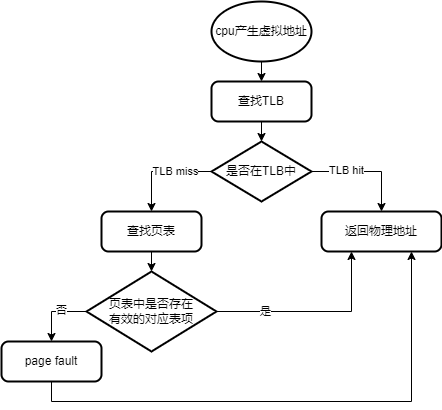
\includegraphics[width=0.5\linewidth]{assets/10/hard-tlb-ctrl.png}
  \caption{基于硬件的TLB管理}
  \label{fig:hard-tlb-ctrl}
\end{figure}

其中，TLB miss后查找页表的这个过程是由硬件自动完成的，软件只需处理后面产生的page fault。整个过程中最多产生一次page fault。

图\ref{fig:soft-tlb-ctrl}则为软件管理TLB方案中虚拟地址转换到物理地址的过程：

\begin{figure}[htbp]
  \centering
  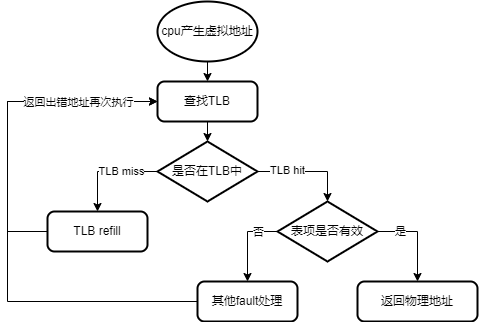
\includegraphics[width=0.5\linewidth]{assets/10/soft-tlb-ctrl.png}
  \caption{基于软件的TLB管理}
  \label{fig:soft-tlb-ctrl}
\end{figure}

具体解释如下：

\begin{enumerate}
\def\labelenumi{\arabic{enumi}.}
\tightlist
\item
  TLB miss后会产生第一次TLB重填（TLB refill）异常，在TLB重填异常中需要软件去遍历页表并填充TLB表项，这里应该是软件管理TLB和硬件管理TLB最大的不同。
\item
  然后TLB重填异常处理中，如果填充的页表项仍然无效，那么在返回后再次查询TLB时，会第二次产生其他的fault处理，以填充页表项、或填充页表项和TLB项。
\item
  如果第二次fault处理中没有重填TLB表项，那么在返回后再次查询TLB时，还会产生第三次TLB重填异常。
\end{enumerate}

可以看到，TLB miss后查找页表的这个过程需要软件进行处理，并且整个过程中最多能产生三次异常。

另外，硬件上会保证在TLB重填异常中不能再次产生TLB重填异常。

\subsection{TLB的软硬件交互机制}\label{sec:10-mmu-004}

TLB的软硬件交互集中体现在TLB相关的异常处理方面，硬件通过异常来处罚相关的软件处理流程，而软件则通过相关指令修复TLB异常。下面结合linux源码对TLB相关异常处理进行分析。

linux中TLB相关异常和相关处理函数的对应关系如下：

\begin{itemize}
\tightlist
\item
  TLB重填异常：handle\_tlb\_refill
\item
  load/取指操作页无效异常：handle\_tlb\_load
\item
  store操作页无效异常：handle\_tlb\_store
\item
  页修改异常：handle\_tlb\_modify
\item
  页不可读/不可写/特权不合规异常：handle\_tlb\_protect
\end{itemize}

这里分析handle\_tlb\_refill、handle\_tlb\_load和handle\_tlb\_protect函数。其中handle\_tlb\_store和handle\_tlb\_modify实际上流程与handle\_tlb\_load基本一致，只是更新页表项时更新的位不同。

\subsubsection{TLB重填异常}\label{sec:10-mmu-005}

TLB重填异常（handle\_tlb\_refill）触发前后硬件中的处理与一般异常存在差异，主要是TLB重填异常相关有独立的一套寄存器。但都会有相应保存和恢复现场、跳转和返回操作。值得注意的是，TLB重填异常中出错的地址保存在CSR.TLBRBADV寄存器，而一般异常出错的地址保存在CSR.BADV寄存器。

TLB重填异常的软件处理过程如下：

\begin{enumerate}
\def\labelenumi{\arabic{enumi}.}
\tightlist
\item
  保存现场
\item
  根据CSR.TLBRBADV中记录的缺失虚拟地址，和CSR.PGD中pgd基址，遍历发生TLB重填异常的进程的多级页表，从内存中取回页表项信息并填入CSR.TLBELO0和CSR.TLBELO1寄存器的相应域中
\item
  根据填入的CSR.TLBELO0和CSR.TLBELO1寄存器信息，最终用tlbfill指令将页表项填入TLB
\item
  恢复并返回
\end{enumerate}

代码分析如下：

% 代码语言：asm
\begin{CodeBlock}
SYM_FUNC_START(handle_tlb_refill)
    csrwr   t0, LOONGARCH_CSR_TLBRSAVE // 将t0保存到CSR.TLBRSAVE寄存器
    csrrd   t0, LOONGARCH_CSR_PGD // 读取pgd基址到t0
    lddir   t0, t0, 3 // 根据CSR.TLBRBADV中记录的缺失虚拟地址，
                      // 访问3级页表，读取2级页表基址到t0（pgd为3级页表基址）
#if CONFIG_PGTABLE_LEVELS > 3
    lddir   t0, t0, 2 // 根据CSR.TLBRBADV中记录的缺失虚拟地址，
                      // 访问2级页表，读取1级页表基址到t0
#endif
#if CONFIG_PGTABLE_LEVELS > 2
    lddir   t0, t0, 1 // 根据CSR.TLBRBADV中记录的缺失虚拟地址，
                      // 访问1级页表，读取末级页表地址或大页到t0
#endif
    ldpte   t0, 0 // 根据CSR.TLBRBADV中记录的缺失虚拟地址，
                  // 访问末级页表或大页，读取偶数号页表项或大页到CSR.TLBELO0
    ldpte   t0, 1 // 根据CSR.TLBRBADV中记录的缺失虚拟地址，
                  // 访问末级页表或大页，读取奇数号页表项或大页到CSR.TLBELO1
    tlbfill // 根据CSR.TLBELO0、CSR.TLBELO1等寄存器中信息，
            // 将页表项填入TLB
    csrrd   t0, LOONGARCH_CSR_TLBRSAVE // 恢复t0
    ertn // 从异常返回
SYM_FUNC_END(handle_tlb_refill)
\end{CodeBlock}

\subsubsection{load/fetch操作页无效异常}\label{sec:10-mmu-006}

load/fetch操作页无效异常触发前后硬件中的处理与一般异常相同。

handle\_tlb\_load处理的过程如下：

\begin{enumerate}
\def\labelenumi{\arabic{enumi}.}
\tightlist
\item
  保存现场
\item
  根据CSR.BADV中记录的缺失虚拟地址，和CSR.PGD中pgd基址，遍历发生异常的进程的多级页表，从内存中取回页表项（或大页）信息
\item
  判断该页表项是否存在，如果不存在则会跳转执行缺页处理函数
\item
  如果存在则将页表项置为有效并填入TLB。最后恢复并返回
\end{enumerate}

代码分析如下：

% 代码语言：asm
\begin{CodeBlock}
SYM_FUNC_START(handle_tlb_load)
    // 将t0、t1、ra写入CSR.SAVE0-CSR.SAVE3，暂存寄存器
    csrwr        t0, EXCEPTION_KS0
    csrwr        t1, EXCEPTION_KS1
    csrwr        ra, EXCEPTION_KS2
    /*
     * The vmalloc handling is not in the hotpath.
     */
    // 如果CSR.BADV不小于0，则继续执行到vmalloc_done_load
    // 将CSR.BADV和CSR.PGDL读入t0和t1
    // 否则跳转到vmalloc_load将CSR.BADV和swapper_pg_dir读入t0和t1
    // 即CSR.BADV不小于0时使用低半部分内核地址的pgd，
    // 否则使用高半部分用户地址的pgd
    csrrd        t0, LOONGARCH_CSR_BADV
    bltz        t0, vmalloc_load
    csrrd        t1, LOONGARCH_CSR_PGDL
vmalloc_done_load:
    /* Get PGD offset in bytes */
    // 根据t0中CSR.BADV地址和t1中pgd基址，遍历页表查找
    bstrpick.d    ra, t0, PTRS_PER_PGD_BITS + PGDIR_SHIFT - 1, PGDIR_SHIFT
    alsl.d        t1, ra, t1, 3
#if CONFIG_PGTABLE_LEVELS > 3
    ld.d        t1, t1, 0
    bstrpick.d    ra, t0, PTRS_PER_PUD_BITS + PUD_SHIFT - 1, PUD_SHIFT
    alsl.d        t1, ra, t1, 3
#endif
#if CONFIG_PGTABLE_LEVELS > 2
    ld.d        t1, t1, 0
    bstrpick.d    ra, t0, PTRS_PER_PMD_BITS + PMD_SHIFT - 1, PMD_SHIFT
    alsl.d        t1, ra, t1, 3
    // 到这里t1中为1级页表（pmd）地址
#endif
    // 将1级页表中第一个表项读取到ra
    ld.d        ra, t1, 0
    /*
     * For huge tlb entries, pmde doesn't contain an address but
     * instead contains the tlb pte. Check the PAGE_HUGE bit and
     * see if we need to jump to huge tlb processing.
     */
    // 如果ra中表项为大页，则跳转到tlb_huge_update_load
    rotri.d        ra, ra, _PAGE_HUGE_SHIFT + 1
    bltz        ra, tlb_huge_update_load

    rotri.d        ra, ra, 64 - (_PAGE_HUGE_SHIFT + 1)
    bstrpick.d    t0, t0, PTRS_PER_PTE_BITS + PAGE_SHIFT - 1, PAGE_SHIFT
    alsl.d        t1, t0, ra, _PTE_T_LOG2
    // 到这里t1中为CSR.BADV对应末级页表项地址

    // 读取页表项到t0
#ifdef CONFIG_SMP
smp_pgtable_change_load:
    ll.d        t0, t1, 0 // smp中使用ll/sc原子指令对循环写入
#else
    ld.d        t0, t1, 0
#endif
    // 如果页表项不存在，则跳转到nopage_tlb_load调用缺页处理函数
    // 否则继续向下执行，写入对应有效的页表项到TLB
    andi        ra, t0, _PAGE_PRESENT
    beqz        ra, nopage_tlb_load

    // 设置有效位并更新页表项
    ori        t0, t0, _PAGE_VALID
#ifdef CONFIG_SMP
    sc.d        t0, t1, 0
    beqz        t0, smp_pgtable_change_load // 写入失败时跳转
#else
    st.d        t0, t1, 0
#endif    
    // 根据CSR.ASID和CSR.TLBEHI的信息查询TLB，以便tlbwr指令写入
    // 如果命中则将其索引写入CSR.TLBIDX，否则将CSR.TLBIDX.NE置为1
    // 这里必然会命中
    tlbsrch

    // t0 = 偶数项页表项，t1 = 奇数项页表项
    bstrins.d    t1, zero, 3, 3
    ld.d        t0, t1, 0
    ld.d        t1, t1, 8
    // 写入TLB相关寄存器
    csrwr        t0, LOONGARCH_CSR_TLBELO0
    csrwr        t1, LOONGARCH_CSR_TLBELO1
    // 根据CSR.TLBELO0、CSR.TLBELO1、CSR.TBLIDX等相关寄存器信息，
    // 将页表项信息写入TLB中CSR.TBLIDX.index对应位置
    tlbwr
    // 恢复并返回
    csrrd        t0, EXCEPTION_KS0
    csrrd        t1, EXCEPTION_KS1
    csrrd        ra, EXCEPTION_KS2
    ertn
#ifdef CONFIG_64BIT
vmalloc_load:
    la.abs        t1, swapper_pg_dir
    b        vmalloc_done_load
#endif
    /* This is the entry point of a huge page. */
tlb_huge_update_load:
    // 对于大页，异常处理的流程和上面基本页表项的处理流程基本一致
    // 只是填入TLB时会做一些额外的格式转换处理等，这里不再赘述
    ...
nopage_tlb_load:
    dbar        0
    csrrd        ra, EXCEPTION_KS2
    la.abs        t0, tlb_do_page_fault_0
    jr        t0
SYM_FUNC_END(handle_tlb_load)
\end{CodeBlock}

\subsubsection{页不可读/不可写/特权不合规异常}\label{sec:10-mmu-007}

页不可读/不可写/特权不合规异常触发前后硬件中的处理与一般异常相同。

handle\_tlb\_protect处理的过程实际上就是调用缺页处理函数，来填入页表。

代码分析如下：

% 代码语言：asm
\begin{CodeBlock}
SYM_FUNC_START(handle_tlb_protect)
    // 保存寄存器
    BACKUP_T0T1
    SAVE_ALL
    // 设置传参
    move    a0, sp
    move    a1, zero
    csrrd    a2, LOONGARCH_CSR_BADV
    REG_S    a2, sp, PT_BVADDR
    // 调用do_page_fault
    la.abs    t0, do_page_fault
    jirl    ra, t0, 0
    // 恢复并返回
    RESTORE_ALL_AND_RET
SYM_FUNC_END(handle_tlb_protect)
\end{CodeBlock}

\section{TLB模块设计}\label{sec:10-mmu-008}

在考虑TLB模块的内部设计时，重点是查找、读和写三套操作的实现。读和写操作可以参考CPU中寄存器文件（regfile）的逻辑设计和Verilog代码实现。本文将主要介绍查找操作的设计实现。

\textbf{读和写操作}

TLB模块的读写接口上的PS域是6比特的，但由于LoongArch精简版中只支持4KB和4MB两种页大小，因此TLB模块内部仅用1比特来存储这两种页大小信息，需要进行一个简单的转换。读和写操作实现可以借鉴CPU寄存器文件的逻辑设计和Verilog代码实现，不再赘述。

\textbf{查找操作}

指令手册中的TLB查找流程伪算法描述是串行化的，但在实际电路实现时，我们并不是先比较第0项、再比较第1项\ldots\ldots 而是同时比较所有项。假设TLB有16项，需要通过组合逻辑产生一个16位宽的查找结果\texttt{match{[}15:0{]}}。这个结果的第0位对应第0项的比较结果，第1位对应第1项的比较结果，以此类推。

下面是查找操作的伪代码示意：

% 代码语言：pseudocode
\begin{CodeBlock}
# 初始TLB未找到标志
tlb_found = 0

# 遍历TLB条目
for i in range(TLB_ENTRIES):
    # 检查当前TLB条目是否有效，且全局标志位为1或ASID匹配，且虚拟页号匹配
    if (TLB[i].E == 1) and ((TLB[i].G == 1) or (TLB[i].ASID == CSR.ASID.ASID)) and \
       (TLB[i].VPPN[VALEN-1: TLB[i].PS+1] == va[VALEN-1: TLB[i].PS+1]):
        
        # 如果之前没有找到匹配的TLB条目
        if tlb_found == 0:
            tlb_found = 1
            found_ps = TLB[i].PS

            # 根据虚拟地址的页偏移选择对应的TLB条目字段
            if va[found_ps] == 0:
                found_v = TLB[i].V0
                found_d = TLB[i].D0
                found_mat = TLB[i].MAT0
                found_plv = TLB[i].PLV0
                found_ppn = TLB[i].PPN0
            else:
                found_v = TLB[i].V1
                found_d = TLB[i].D1
                found_mat = TLB[i].MAT1
                found_plv = TLB[i].PLV1
                found_ppn = TLB[i].PPN1
        else:
            # 出现多项命中，处理器运行结果不确定
            # 这里可能需要添加相关处理逻辑

# 如果没有找到匹配的TLB条目，触发TLB重填例外
if tlb_found == 0:
    SignalException(TLBR)

# 如果找到的条目无效，根据访问类型触发相应的例外
if found_v == 0:
    if mem_type == 'FETCH':
        SignalException(PIF)  # 取指操作页无效例外
    elif mem_type == 'LOAD':
        SignalException(PIL)  # 读取操作页无效例外
    elif mem_type == 'STORE':
        SignalException(PIS)  # 存储操作页无效例外

# 如果访问的特权等级超过页表项的特权等级，触发页特权等级不合规例外
elif plv > found_plv:
    SignalException(PPI)

# 如果是存储操作且页面未修改，触发页修改例外
elif mem_type == 'STORE' and found_d == 0:
    SignalException(PME)

# 否则计算物理地址并设置内存属性
else:
    pa = {found_ppn[PALEN-13:found_ps-12], va[found_ps-1:0]}
    mat = found_mat

\end{CodeBlock}

要生成查询比较结果，首先需确定是否命中。这可以通过检查匹配结果是否全为零来判断。如果匹配结果不全为零，则表示有命中项。命中项的物理页号（PFN）等信息的读取逻辑也相对简单。

接下来，我们分析INVTLB指令所需的查找操作支持。由于当前TLB实现采用并行查找机制进行虚拟地址到物理地址的转换，因此INVTLB指令的查找也将采用并行查找机制，即同时对TLB中的各项进行匹配判断。设计的关键在于如何处理每一项的匹配。通过分析INVTLB指令的操作定义，我们可以将各操作的匹配分解为若干``子匹配''逻辑组合。具体来说，有四个``子匹配''的判断条件：

\begin{enumerate}
\def\labelenumi{\arabic{enumi}.}
\item
  cond1------G域是否等于0；
\item
  cond2------G域是否等于1；
\item
  cond3------s1\_asid是否等于ASID域；
\item
  cond4------s1\_vppn是否匹配VPPN和PS域。
\end{enumerate}

在此基础上，不同操作的匹配条件可以表达如下：

\begin{itemize}
\tightlist
\item
  对于op=0和op=1，匹配条件为cond1或cond2；
\item
  对于op=4，匹配条件为cond1且cond3；
\item
  对于op=5，匹配条件为cond1且cond3且cond4；
\item
  对于op=6，匹配条件为（cond2或cond3）且cond4。
\end{itemize}

值得注意的是，op=6的匹配条件正是取指和访存进行虚实地址转换时的查找匹配条件，因此这两类操作的查找匹配功能可以统一到同一逻辑中。两者的区别仅在于基于查找结果所采取的进一步操作。对于INVTLB指令，将相应TLB表项无效化的操作是将inv\_match{[}i{]}等于1对应的tlb\_e{[}i{]}置为0。

\section{TLB相关的寄存器与指令}\label{sec:10-mmu-009}

\subsection{TLB相关的CSR寄存器}\label{sec:10-mmu-010}

在LoongArch架构下，关于TLB（转换后备缓冲区）相关的控制状态寄存器（CSR）有以下几个重要的寄存器：

\begin{enumerate}
\def\labelenumi{\arabic{enumi}.}
\tightlist
\item
  \textbf{CSR.ASID}：这是地址空间标识符寄存器，用于标识不同的地址空间。每个TLB条目与一个特定的ASID相关联，这样可以在不清空TLB的情况下进行上下文切换。
\item
  \textbf{CSR.TLBEHI}：TLB入口高位寄存器，存储虚拟地址的高位部分以及其他一些控制信息。用于查询和操作TLB条目时提供所需的地址信息。
\item
  \textbf{CSR.TLBELO0 和 CSR.TLBELO1}：这两个寄存器分别存储TLB条目的低位部分，包括物理地址和页表项的其他标志。TLBELO0和TLBELO1分别对应一个TLB条目的两个物理页框地址。
\item
  \textbf{CSR.TLBIDX}：这是TLB索引寄存器，包含用于指定TLB条目索引的字段。还包括一个指示TLB条目是否有效的标志位（INV）。
\end{enumerate}

更详细的介绍请参看LoongArch精简指令集手册。

\subsection{TLB相关的指令}\label{sec:10-mmu-011}

以下表格总结了LoongArch指令集架构中用于TLB管理和维护的指令：

\begin{longtable}[]{@{}
  >{\raggedright\arraybackslash}p{(\linewidth - 4\tabcolsep) * \real{0.0870}}
  >{\raggedright\arraybackslash}p{(\linewidth - 4\tabcolsep) * \real{0.5217}}
  >{\raggedright\arraybackslash}p{(\linewidth - 4\tabcolsep) * \real{0.3913}}@{}}
\toprule\noalign{}
\begin{minipage}[b]{\linewidth}\raggedright
指令
\end{minipage} & \begin{minipage}[b]{\linewidth}\raggedright
描述
\end{minipage} & \begin{minipage}[b]{\linewidth}\raggedright
使用示例
\end{minipage} \\
\midrule\noalign{}
\endhead
\bottomrule\noalign{}
\endlastfoot
\texttt{tlbsrch} & 查询TLB对应的索引。使用CSR.ASID和CSR.TLBEHI中的信息查询TLB，如果命中则将其对应索引写入CSR.TLBIDX.Index，否则将CSR.TLBIDX.NE置为1。 & \texttt{tlbsrch}指令查询TLB中是否包含特定的页表项。 \\
\texttt{tlbrd} & 读取索引对应的TLB表项。将CSR.TLBIDX.Index作为索引，读取TLB中的指定项。如果该TLB项有效，则将其页表项信息写入CSR.TLBEHI、CSR.TLBELO0、CSR.TLBELO1和CSR.TLBINX.PS寄存器，并将CSR.TLBIND.NE置0；如果无效，则将CSR.TLBIND.NE置1。 & \texttt{tlbrd}指令读取TLB中的特定表项信息。 \\
\texttt{tlbwr} & 写入索引对应的TLB表项。将CSR.TLBIDX.Index作为索引，把CSR.TLBEHI、CSR.TLBELO0、CSR.TLBELO1和CSR.TLBINX.PS中的页表项信息写入TLB中的指定项。如果CSR.TLBIND.NE置为1，则写入的是一个无效的TLB项。 & \texttt{tlbwr}指令将页表项信息写入TLB中的指定位置。 \\
\texttt{tlbfill} & 类似于\texttt{tlbwr}指令，不同的是\texttt{tlbfill}写入TLB位置由硬件随机决定。 & \texttt{tlbfill}指令随机插入页表项到TLB中。 \\
\texttt{tlbclr} & 根据TLB相关CSR中的信息无效化TLB中的内容。 & \texttt{tlbclr}指令无效化TLB中的特定表项。 \\
\texttt{tlbflush} & 根据TLB相关CSR中的信息无效化TLB中的内容，但作用范围较\texttt{tlbclr}更广。 & \texttt{tlbflush}指令无效化TLB中的所有表项。 \\
\texttt{invtlb} & 用于无效化TLB中的内容，比\texttt{tlbclr}和\texttt{tlbflush}指令更加灵活。 & \texttt{invtlb}指令用于灵活地无效化TLB中的特定表项。 \\
\end{longtable}

\section{利用TLB进行虚实地址转换}\label{sec:10-mmu-012}

\subsection{地址翻译}\label{sec:10-mmu-013}

下面我们主要介绍LoongArch架构下是如何进行虚拟地址翻译的。

\subsubsection{地址空间}\label{sec:10-mmu-014}

在LoongArch架构中，虚拟地址空间和物理地址空间的大小如下：

\textbf{虚拟地址空间}

\begin{itemize}
\tightlist
\item
  \textbf{LA32}：虚拟地址空间大小为 2\textsuperscript{32} 字节。
\item
  \textbf{LA64}：虚拟地址空间大小为 2\textsuperscript{64} 字节。
\end{itemize}

\textbf{物理地址空间}

\begin{itemize}
\tightlist
\item
  \textbf{LoongArch中的物理地址空间大小为} 2\textsuperscript{PALEN} 字节，其中：

  \begin{itemize}
  \tightlist
  \item
    \textbf{LA32}：PALEN为一个不超过36的正整数，通常为32。
  \item
    \textbf{LA64}：PALEN为一个不超过60的正整数。
  \end{itemize}
\end{itemize}

PALEN由具体实现决定，软件可以通过CPUCFG指令读取PALEN的值。

\subsubsection{地址翻译模式}\label{sec:10-mmu-015}

loongarch中通过控制寄存器CSR.CRMD配置地址翻译模式：

\begin{itemize}
\tightlist
\item
  CSR.CRMD中DA=1且PG=0：直接地址翻译模式
\item
  CSR.CRMD中DA=0且PG=1：映射地址翻译模式
\item
  其他DA和PG值的组合的行为未定义
\end{itemize}

下表是这两个寄存器的详细定义

\begin{longtable}[]{@{}
  >{\raggedright\arraybackslash}p{(\linewidth - 6\tabcolsep) * \real{0.0556}}
  >{\raggedright\arraybackslash}p{(\linewidth - 6\tabcolsep) * \real{0.0556}}
  >{\raggedright\arraybackslash}p{(\linewidth - 6\tabcolsep) * \real{0.0556}}
  >{\raggedright\arraybackslash}p{(\linewidth - 6\tabcolsep) * \real{0.8333}}@{}}
\toprule\noalign{}
\begin{minipage}[b]{\linewidth}\raggedright
位
\end{minipage} & \begin{minipage}[b]{\linewidth}\raggedright
名称
\end{minipage} & \begin{minipage}[b]{\linewidth}\raggedright
RW
\end{minipage} & \begin{minipage}[b]{\linewidth}\raggedright
描述
\end{minipage} \\
\midrule\noalign{}
\endhead
\bottomrule\noalign{}
\endlastfoot
3 & DA & RW & 直接地址翻译模式的使能，高有效。\newline{}当触发 TLB 重填例外时，硬件将该域置为 1。\newline{}当执行 ERTN 指令从例外处理程序返回时，如果 CSR.ESTAT.Ecode=0x3F，则硬件将该域置为 0。\newline{}DA 位和 PG 位的合法组合情况为 0, 1 或 1, 0，当软件配置成其它组合情况时结果不确定。 \\
4 & PG & RW & 映射地址翻译模式的使能，高有效。\newline{}当触发 TLB 重填例外时，硬件将该域置为 0。\newline{}当执行 ERTN 指令从例外处理程序返回时，如果 CSR.ESTAT.Ecode=0x3F，则硬件将该域置为 1。\newline{}PG 位和 DA 位的合法组合情况为 0, 1 或 1, 0，当软件配置成其它组合情况时结果不确定。 \\
\end{longtable}

LoongArch架构中的虚实地址转换机制由其地址翻译模式确定。LoongArch中有以下两种地址翻译模式：

\begin{enumerate}
\def\labelenumi{\arabic{enumi}.}
\item
  \textbf{直接地址翻译模式}：

  \begin{itemize}
  \tightlist
  \item
    在该模式下，物理地址直接等于虚拟地址的低PALEN位，不足部分补0。此模式相当于没有进行映射。
  \end{itemize}
\item
  \textbf{映射地址翻译模式}：

  \begin{itemize}
  \tightlist
  \item
    该模式下又分为两种子模式：

    \begin{itemize}
    \item
      \textbf{直接映射地址翻译模式（直接映射模式）}：

      LoongArch中的直接映射模式是一种线性的映射方式，有点类似于分段。通过配置直接映射配置窗口寄存器，可以实现直接映射。

      共有4个直接映射配置窗口寄存器，分别为CSR.DMW0到CSR.DMW3。配置一个窗口相当于映射一段内存区域。其中：

      \begin{itemize}
      \tightlist
      \item
        \textbf{CSR.DMW0}和\textbf{CSR.DMW1}：

        \begin{itemize}
        \tightlist
        \item
          映射的内存区域可以同时用于取指和load/store操作。
        \end{itemize}
      \item
        \textbf{CSR.DMW2}和\textbf{CSR.DMW3}：

        \begin{itemize}
        \tightlist
        \item
          映射的内存区域仅用于load/store操作。
        \end{itemize}
      \end{itemize}

      通过这些配置窗口寄存器，用户可以灵活地定义虚拟地址到物理地址的直接映射区域，以满足不同的内存访问需求。
    \item
      \textbf{页表映射地址翻译模式（页表映射模式）}：

      在LoongArch架构中，可以同时有两个页全局目录（PGD）基址，这两个基址分别存储于寄存器CSR.PGDL（低半地址空间全局目录基址）和CSR.PGDH（高半地址空间全局目录基址），分别对应低半地址空间和高半地址空间。低半地址空间和高半地址空间实际上是将虚拟地址空间对半分成两个部分：

      \begin{itemize}
      \tightlist
      \item
        \textbf{低半地址空间}：

        \begin{itemize}
        \tightlist
        \item
          虚拟地址的最高位为0。
        \item
          使用CSR.PGDL中的基址进行地址转换。
        \end{itemize}
      \item
        \textbf{高半地址空间}：

        \begin{itemize}
        \tightlist
        \item
          虚拟地址的最高位为1。
        \item
          使用CSR.PGDH中的基址进行地址转换。
        \end{itemize}
      \end{itemize}

      两个部分的地址转换互不干扰，各自使用对应的PGD。在Linux中：

      \begin{itemize}
      \tightlist
      \item
        \textbf{CSR.PGDH}：存放内核进程的PGD。
      \item
        \textbf{CSR.PGDL}：存放用户进程的PGD。
      \end{itemize}

      这种设计在硬件上实现了对内核空间和用户空间的页表隔离，提高了系统的安全性和稳定性。
    \end{itemize}
  \end{itemize}
\end{enumerate}

\textbf{总之：}

直接地址翻译模式和映射地址翻译模式不能同时启用。在映射地址翻译模式下，可以同时启用直接映射模式和页表映射模式。在进行地址翻译时，系统会优先使用直接映射模式，如果无法使用直接映射模式，则使用页表映射模式进行翻译。

LoongArch架构的地址翻译机制通过配置不同的地址翻译模式实现虚拟地址到物理地址的转换，具有灵活性和高效性。通过合理配置CSR.CRMD寄存器中的DA和PG位，用户可以根据需求选择直接地址翻译模式或映射地址翻译模式，从而实现不同的内存访问需求和系统性能优化。

\subsection{TLB接口设计}\label{sec:10-mmu-016}

页表映射模式的核心组件便是TLB，通过梳理TLB模块相关知识，并结合CPU流水线的结构特点，我们对TLB模块的设计分析如下：

\begin{enumerate}
\def\labelenumi{\arabic{enumi}.}
\tightlist
\item
  \textbf{查找表结构}：

  \begin{itemize}
  \tightlist
  \item
    TLB模块的主体应为一个二维组织结构的查找表。每一项分为两部分：

    \begin{itemize}
    \tightlist
    \item
      第一部分存储的信息既参与读写又参与查找比较，包括E、VPPN、PS、ASID和G。
    \item
      第二部分仅参与读写，包括PPN0、PLV0、MAT0、D0、V0、PPN1、PLV1、MAT1、D1、V1。
    \end{itemize}
  \item
    查找表的项数由实现者自行定义。
  \end{itemize}
\item
  \textbf{虚实地址转换支持}：

  \begin{itemize}
  \tightlist
  \item
    TLB模块要支持取指和访存的虚实地址转换需求，两个部分都需要对TLB模块进行查找，且查找功能一致。
  \item
    查找时，向TLB模块输入s\_vppn、s\_va\_bit12和s\_asid信息，输出信息包括s\_found、s\_ppn、s\_ps、s\_plv、s\_mat、s\_d和s\_v。
  \item
    输入信息：

    \begin{itemize}
    \tightlist
    \item
      s\_vppn来自访存虚地址的31..13位，
    \item
      s\_va\_bit12来自访存虚地址的12位，
    \item
      s\_asid来自CSR.ASID的ASID域。
    \end{itemize}
  \item
    输出信息：

    \begin{itemize}
    \tightlist
    \item
      s\_ppn和s\_ps用于产生最终的物理地址，
    \item
      s\_found用于判定是否产生TLB重填异常，
    \item
      s\_found和s\_v用于判定是否产生页无效异常，
    \item
      s\_found和s\_plv用于判定是否产生页特权等级不合规异常，
    \item
      s\_found、s\_v和s\_d用于判定是否产生页修改异常。
    \end{itemize}
  \end{itemize}
\item
  \textbf{并行查找支持}：

  \begin{itemize}
  \tightlist
  \item
    为了使流水线能够满负荷运转不断流，TLB模块要能够支持取指和访存同时进行查找。这意味着查找端口应该有两套。
  \end{itemize}
\item
  \textbf{TLBSRCH指令支持}：

  \begin{itemize}
  \tightlist
  \item
    TLB模块需要支持TLBSRCH指令的查找操作，建议复用访存指令查找TLB的端口，输入复用s\_vppn和s\_asid，输出复用已有的s\_found。
  \item
    需要一个额外的s\_index输出，用于记录命中在第几项，其信息用于填入到CSR.TLBIDX中。
  \end{itemize}
\item
  \textbf{TLBWR和TLBFILL指令支持}：

  \begin{itemize}
  \tightlist
  \item
    TLB模块需要支持TLBWR和TLBFILL指令的写操作，建议为此设计独立的端口。
  \item
    输入信息包括写地址w\_index，写入的TLB表项信息w\_e、w\_vppn、w\_ps、w\_asid、w\_g、w\_ppn0、w\_plv0、w\_mat0、w\_d0、w\_v0、w\_ppn1、w\_plv1、w\_mat1、w\_d1、w\_v1。
  \item
    写操作需有写使能输入信号we。
  \end{itemize}
\item
  \textbf{TLBRD指令支持}：

  \begin{itemize}
  \tightlist
  \item
    TLB模块需要支持TLBRD指令的读操作，建议为此设计独立的端口。
  \item
    输入信息包括读地址r\_index。
  \item
    输出结果有r\_e、r\_vppn、r\_ps、r\_asid、r\_g、r\_ppn0、r\_plv0、r\_mat0、r\_d0、r\_v0、r\_ppn1、r\_plv1、r\_mat1、r\_d1、r\_v1。
  \end{itemize}
\item
  \textbf{INVTLB指令支持}：

  \begin{itemize}
  \tightlist
  \item
    TLB模块需要支持INVTLB指令的查找和无效操作。
  \item
    不同操作类型的查找信息可复用访存指令查找TLB的端口，仅需一个额外的invtlb\_op输入，用于标识具体操作类型。
  \item
    invtlb的无效操作在TLB模块内部根据查找结果直接将符合条件的TLB表项的E位置为0。
  \end{itemize}
\end{enumerate}

通过上述分析，我们得到TLB模块的接口与内部主要信号的定义如下：

% 代码语言：verilog
\begin{CodeBlock}
module tlb
#(
    parameter TLBNUM = 16
)
(
    input  wire                      clk,

    // search port 0 (for fetch)
    input  wire [              18:0] s0_vppn,
    input  wire                      s0_va_bit12,
    input  wire [               9:0] s0_asid,
    output wire                      s0_found,
    output wire [$clog2(TLBNUM)-1:0] s0_index,
    output wire [              19:0] s0_ppn,
    output wire [               5:0] s0_ps,
    output wire [               1:0] s0_plv,
    output wire [               1:0] s0_mat,
    output wire                      s0_d,
    output wire                      s0_v,

    // search port 1 (for load/store)
    input  wire [              18:0] s1_vppn,
    input  wire                      s1_va_bit12,
    input  wire [               9:0] s1_asid,
    output wire                      s1_found,
    output wire [$clog2(TLBNUM)-1:0] s1_index,
    output wire [              19:0] s1_ppn,
    output wire [               5:0] s1_ps,
    output wire [               1:0] s1_plv,
    output wire [               1:0] s1_mat,
    output wire                      s1_d,
    output wire                      s1_v,

    // invtlb opcode
    input  wire                      invtlb_valid,
    input  wire [               4:0] invtlb_op,

    // write port
    input  wire                      we,     //w(rite) e(nable)
    input  wire [$clog2(TLBNUM)-1:0] w_index,
    input  wire                      w_e,
    input  wire [              18:0] w_vppn,
    input  wire [               5:0] w_ps,
    input  wire [               9:0] w_asid,
    input  wire                      w_g,
    input  wire [              19:0] w_ppn0,
    input  wire [               1:0] w_plv0,
    input  wire [               1:0] w_mat0,
    input  wire                      w_d0,
    input  wire                      w_v0,
    input  wire [              19:0] w_ppn1,
    input  wire [               1:0] w_plv1,
    input  wire [               1:0] w_mat1,
    input  wire                      w_d1,
    input  wire                      w_v1,

    // read port
    input  wire [$clog2(TLBNUM)-1:0] r_index,
    output wire                      r_e,
    output wire [              18:0] r_vppn,
    output wire [               5:0] r_ps,
    output wire [               9:0] r_asid,
    output wire                      r_g,
    output wire [              19:0] r_ppn0,
    output wire [               1:0] r_plv0,
    output wire [               1:0] r_mat0,
    output wire                      r_d0,
    output wire                      r_v0,
    output wire [              19:0] r_ppn1,
    output wire [               1:0] r_plv1,
    output wire [               1:0] r_mat1,
    output wire                      r_d1,
    output wire                      r_v1
);

reg  [TLBNUM-1:0] tlb_e;
reg  [TLBNUM-1:0] tlb_ps4MB; //pagesize 1:4MB, 0:4KB
reg  [      18:0] tlb_vppn     [TLBNUM-1:0];
reg  [       9:0] tlb_asid     [TLBNUM-1:0];
reg               tlb_g        [TLBNUM-1:0];
reg  [      19:0] tlb_ppn0     [TLBNUM-1:0];
reg  [       1:0] tlb_plv0     [TLBNUM-1:0];
reg  [       1:0] tlb_mat0     [TLBNUM-1:0];
reg               tlb_d0       [TLBNUM-1:0];
reg               tlb_v0       [TLBNUM-1:0];
reg  [      19:0] tlb_ppn1     [TLBNUM-1:0];
reg  [       1:0] tlb_plv1     [TLBNUM-1:0];
reg  [       1:0] tlb_mat1     [TLBNUM-1:0];
reg               tlb_d1       [TLBNUM-1:0];
reg               tlb_v1       [TLBNUM-1:0];

......

endmodule
\end{CodeBlock}
